\begin{problem}{两只脑斧}{standard input}{standard output}{1 second}{128 megabytes}

    天天最近想要学习用口琴给筝筝吹情歌,但是他以前从来没有学过口琴,只能从最简单的两只脑斧开始学。而口琴有时吸气有时吹气的吹法让天天傻傻地分不清,所以他就只能拿着乐谱来找聪明的你了,快帮帮他!

    \begin{center}
        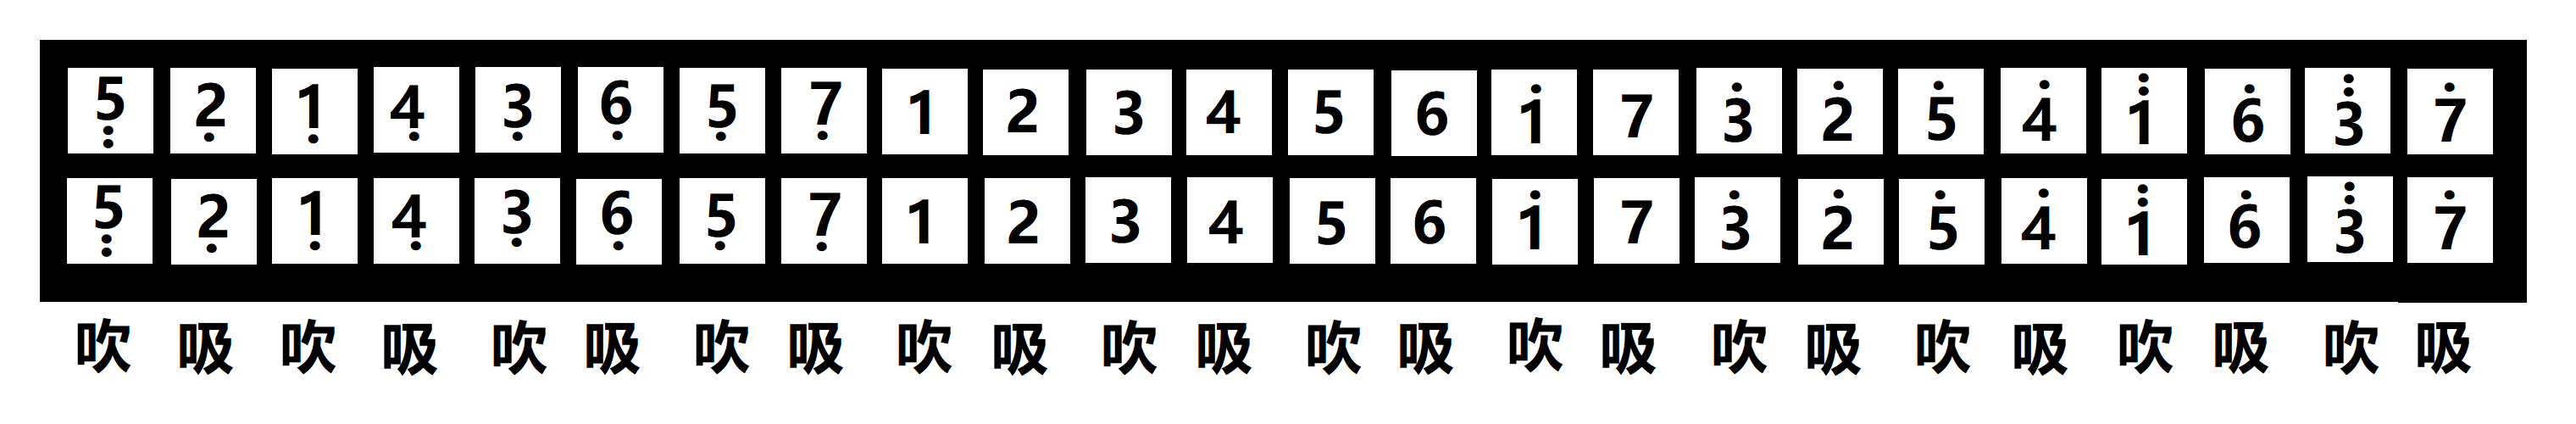
\includegraphics[width=17cm]{Official/1.png}
    \end{center}

    已知天天使用的是 $24$ 孔口琴,其音阶图如上,其中 $1,2,\cdots,7$ 七个阿拉伯数字表示基本的音阶,数字上方有\texttt{.}或\ \texttt{:}的音阶则分别表示该音阶的音调将在原音阶基础上增高一个八度或两个八度,例如音阶 $3$ 的高八度为 $\overset{.}{3}$。相应的,数字下方有\texttt{.}或\ \texttt{:}的音阶也分别表示降低一个八度或两个八度的音调,例如音阶 $5$ 的低二八度为 $\underset{:}{5}$。

    \InputFile

    输入共两行,第一行输入一个正整数 $n\ (1\le n\le 100)$,表示乐谱中有 $n$ 个音符。

    第二行输入 $n$ 个由空格间隔开的字符串,每个字符串描述该乐谱中的一个音阶,这里使用符号\texttt{+}和\texttt{-}来分别表示音阶地高八度和低八度,例如上图的口琴乐谱的第一个音阶和最后一个音阶可以分别用\texttt{5-}\texttt{-}和\texttt{7+}来表示。
    
    \OutputFile
    
    请输出 $n$ 个字符描述的口琴吹法,其中第 $i$ 个字符将描述第 $i$ 个音阶的吹法,请用\texttt{I}表示吸气,用\texttt{E}表示吹气,用\texttt{X}表示停顿(在简谱中用\texttt{0}表示)。
    
    \Example
    
    \begin{example}
    \exmp{
        34
        1 2 3 1 1 2 3 1 3 4 5 3 4 5 5 6 5 4 3 1 5 6 5 4 3 1 2 5- 1 0 2 5- 1 0

    }{
        EIEEEIEEEIEEIEEIEIEEEIEIEEIEEXIEEX
    }%
    \end{example}

\end{problem}